% Created:  
% Author:   Julie Sewards
% Filename: implementation.tex

\chapter{Implementation}
\label{cha:imp}
\section{Development Environment}
An early challenge encountered in this project was setting up a suitable development environment.  Initially the intention was to use the Android Development Tools plug-in for Eclipse, as this was an extension to an already familiar IDE, however, difficulties were encountered with the school computers and finally we elected to switch to Android Studio (Beta) as suggested on the Android Developers website \cite{android_dev}.  

Since the main rationale for the Android application was to allow users to read documents away from the PC, we felt that the application should be optimised for use on a tablet.  As a difficulty arose in getting the device emulators to work on Linux, it became necessary to purchase a physical device for the purposes of the project.  Budget too was a significant consideration; therefore the device chosen was a Hudl 7" tablet running the Android 4.2.2 Jelly Bean operating system.  For the purposes of this project, it was decided that we would develop and test for this device.  This meant that we were restricted to API 17, which eliminated the need to include any backward compatibility but also precluded using features of the latest Android releases as it transpired that there was no upgrade path available for this device.  This fact turned out to be highly significant in a later stage of the project.  

\section{Initial Development}
It was felt wise to begin by developing a very simple application in order to gain some familiarity with the complexities of the Android architecture and its API. This initial application enabled us to input some text, encrypt it (using "convert to upper case" in lieu of encryption) and write it to the application storage.  

The next stage was to introduce actual encryption, for which we needed to investigate the Java Cryptography Architecture(JCA).  Although the choice of algorithm was determined as part of the design, we were mindful of the fact that  many security weaknesses are introduced by poor implementation. As \cite{schneier1998security} states,
\begin{quotation}
'And just as it's possible to build a weak structure using strong materials, it's possible to build a weak cryptographic system using strong algorithms and protocols' 
\end{quotation}  
For this reason we decided that we would initially develop and test the  Java classes to be used for encryption and decryption in the more familiar Linux environment before porting to Android.  Linux also provides a simple command line interface which was valuable for inspecting the binary (or hex) content of encrypted files to aid debugging.

\section{SecurelyShare Prototype}
In undertaking this project we were keen to understand more of the tools and techniques of Android development, therefore we attempted to incorporate a number different user interface components including altert and custom dialogs, fragments and ActionBar menus.
\subsection*{Initialisation}

The Initialisation Activity is run the first time SecurelyShare is installed.  The user is asked whether they wish to import a KeyStore from backup and asked to set up a master password.  In the current implementation, the import option must be chosen as the Certificate keystore needs to be created on a PC, either in Linux using  \texttt{keytool} from the command line or using a program called \texttt{Portecle}  \cite{portecle}.  An empty keystore is created for the group keys and the user is asked to confirm to proceed.  We used 

\begin{figure}[h!]
    \centering
    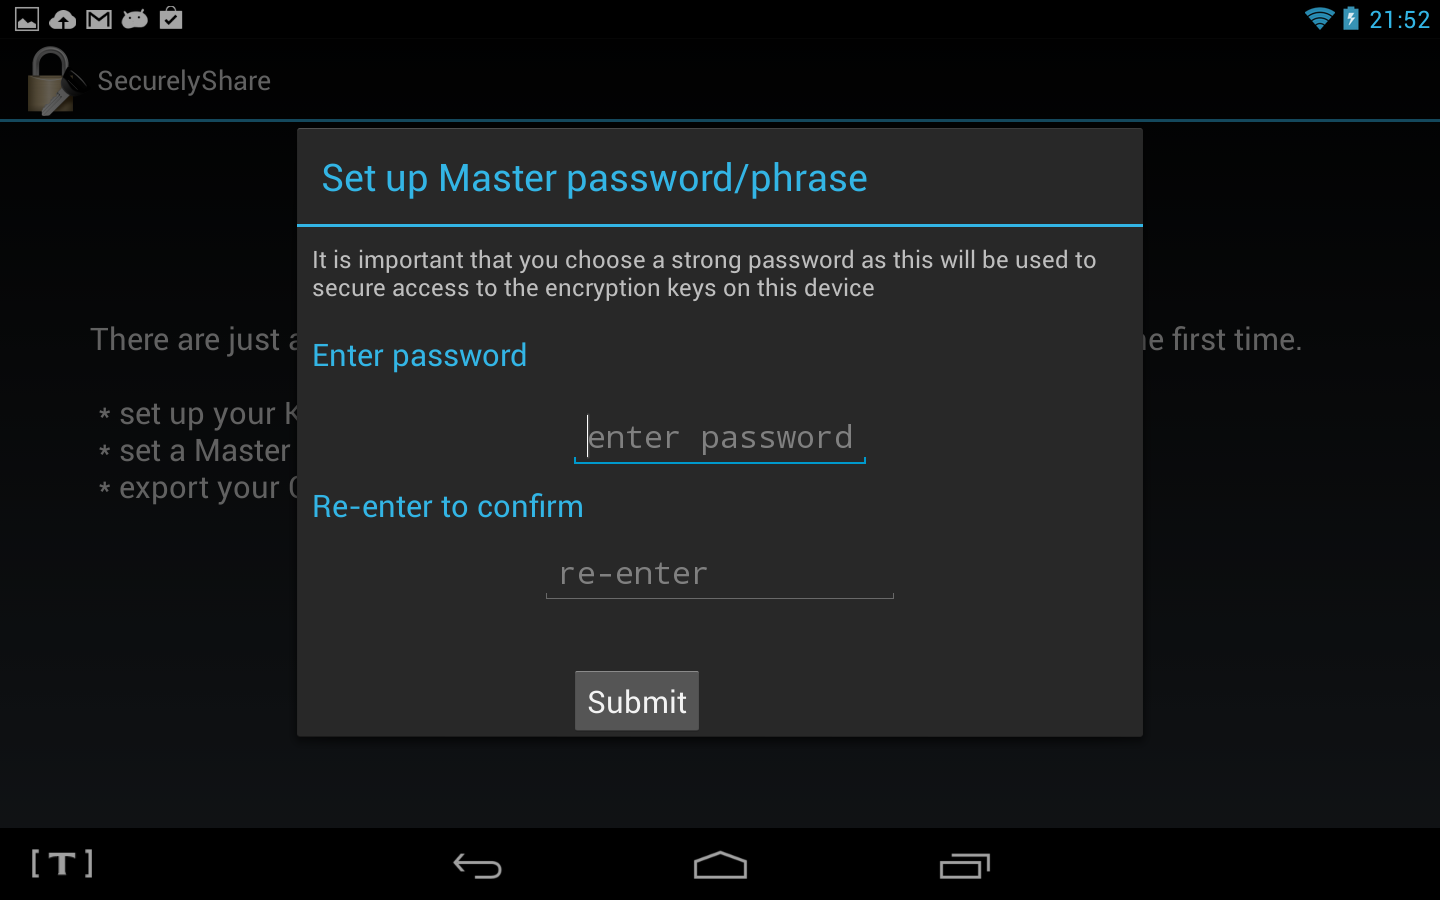
\includegraphics[width=0.5\textwidth]{Setup}                                                                                                                                                                                                                                                                                                                                                                                                                                                                                                                                                                                                                                                                                                                                                                                                                                                                                                                                                                                                                                                                                                                                                                                                                                                                                                                                                                                                                                                                                                                                                                                                                                                                                                                                                                                                                                                                                                                                                                                                                                                                                                                                                                                                                                                                                                                                                                                                                                                                                                                                                                                                                                                                                                                                                                                                                                                                                                                                                                          
    \caption{Set Master Password }
    \label{fig:alert}
\end{figure}

\subsection*{Main Activity}
The home page consists simply of four buttons for loving to the other main activities in SecurelyShare.  We recognise that this is somewhat visually unappealing and duplicates the menu options included in the Action Bar, however, in line with our design goals, it was felt better to focus on improving security features rather than visual appeal at this stage.

The user is invited to enter the Master password upon opening the application and, having decided that we would not require the password to be re-entered to access each file, it was necessary to ensure that this data was available wherever needed.  Researching the various developer forums to see if there was any accepted good practice revealed this to be a contentious question.  Although a popular approach, writing data to the  \textt{SharedPreference} database as a means of passing it between applications represents poor practice, (particularly so when this data is a password).  More experiened developers were divided as to whether this was best done by extending the \textt{Application} class or by use of the Singleton design pattern.  
\begin{figure}[h!]
    \centering
    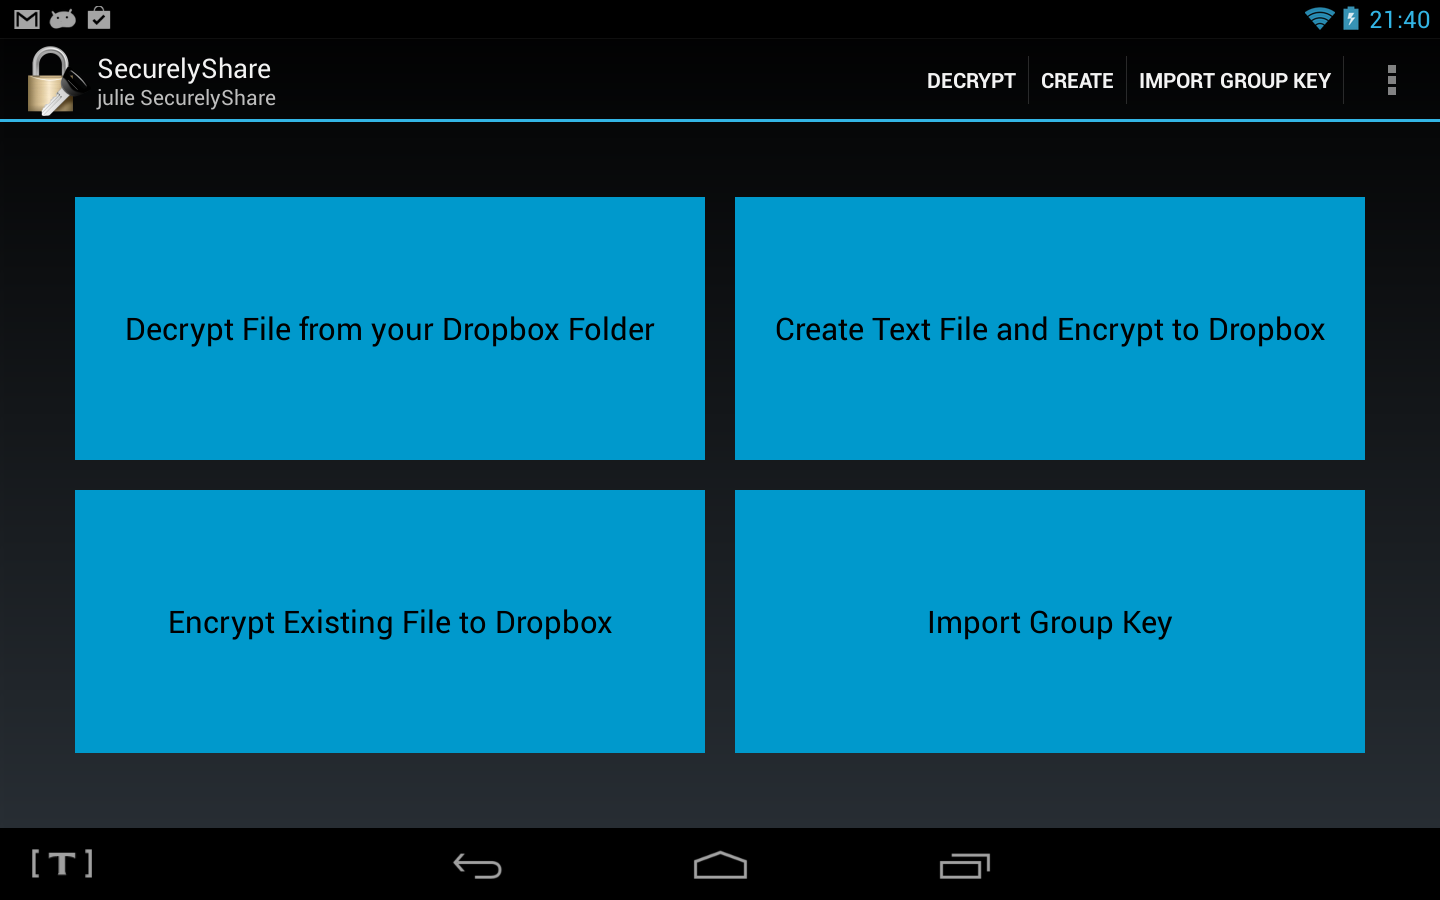
\includegraphics[width=0.5\textwidth]{main}                                                                                                                                                                                                                                                                                                                                                                                                                                                                                                                                                                                                                                                                                                                                                                                                                                                                                                                                                                                                                                                                                                                                                                                                                                                                                                                                                                                                                                                                                                                                                                                                                                                                                                                                                                                                                                                                                                                                                                                                                                                                                                                                                                                                                                                                                                                                                                                                                                                                                                                                                                                                                                                                                                                                                                                                                                                                                                                                                                          
    \caption{Basic home screen}
    \label{fig:main}
\end{figure}

\begin{figure}[h!]
    \centering
    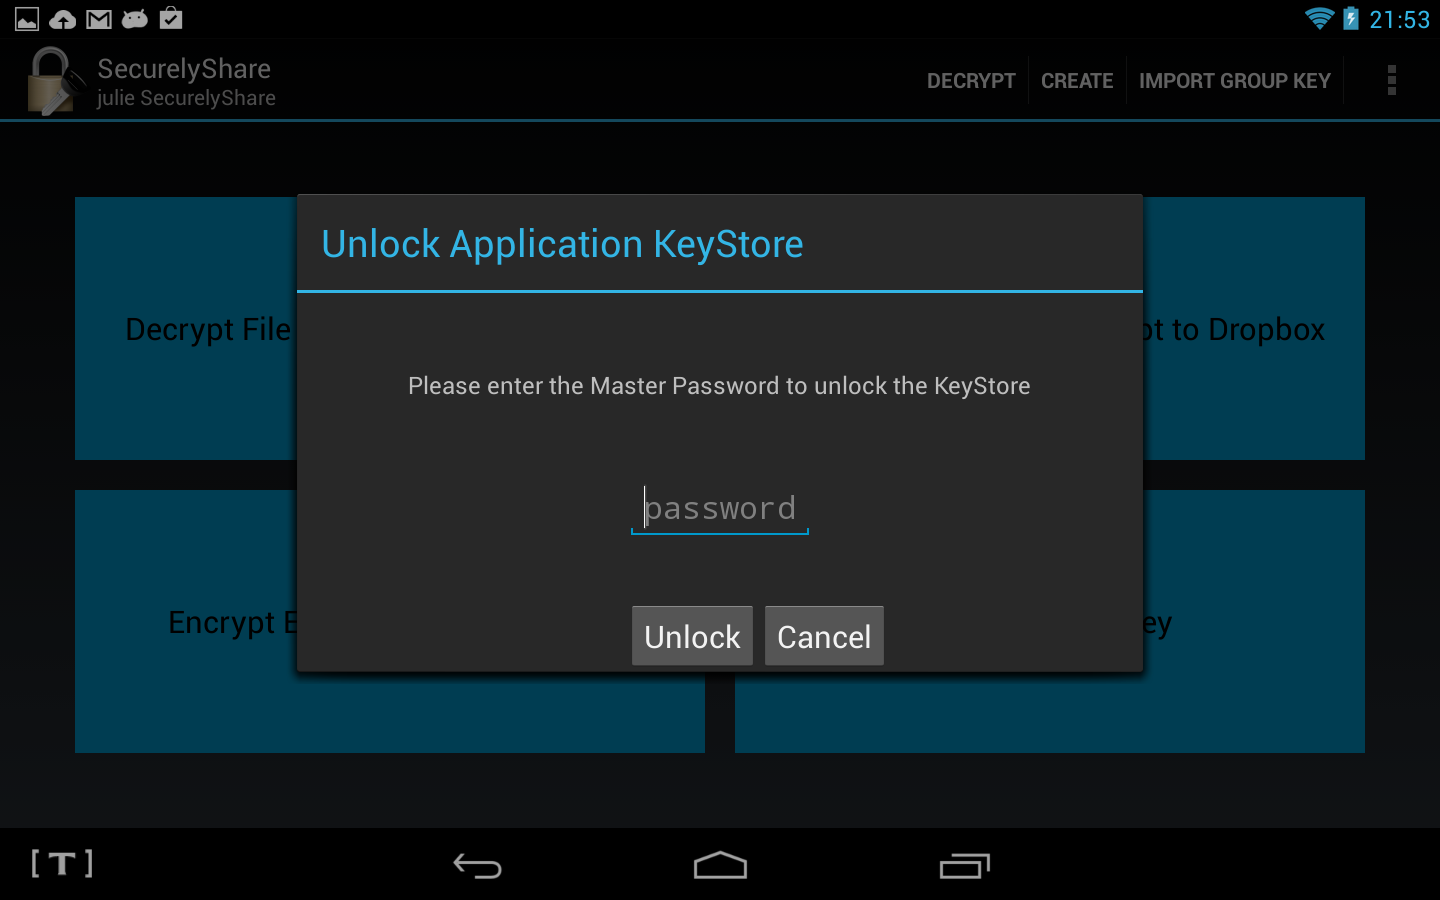
\includegraphics[width=0.5\textwidth]{Unlock}                                                                                                                                                                                                                                                                                                                                                                                                                                                                                                                                                                                                                                                                                                                                                                                                                                                                                                                                                                                                                                                                                                                                                                                                                                                                                                                                                                                                                                                                                                                                                                                                                                                                                                                                                                                                                                                                                                                                                                                                                                                                                                                                                                                                                                                                                                                                                                                                                                                                                                                                                                                                                                                                                                                                                                                                                                                                                                                                                                          
    \caption{Dialog to request Master password to unlock access to KeyStores }
    \label{fig:unlock}
\end{figure}





\section{Implementation Challenges}
One aspect of the Android environment which is challenging for newcomers is the way in which the operating system actively manages storage.  When the user navigates away from an activity, it operating system holds it in memory in a paused state.  If, however, memory resources run short, the current instance of the activity is simply destroyed and a new one created next time the user navigates back to it, causing variables to be reinitialised.


DROPBOX
For improvement, use custom file extension registered with Dropbox then would only ever see encrypted files

GOOD PRACTICE
use of bundle for passing data between activities

use of interface for passing data back from dialog

Use of singleton



ANDROID FEATURES

Splash screen and initialization

Fragments

Implemented with algorithms as static variables so that easy to amend if standards change

CRYPTOGRAPHY




CHALLENGES
Major issues with keystore, certificates and default providers.

dbx stuff does not implement serialisable or parcelable


Challenge of unavailability of BKS on pcs in school

No access to key tool in android

Issue: if generate [private key on device, it is device specific - ability to import would allow same keystores to be used on multiple devices for4 same user


Issue: if generate [rivate key on device, it is device specific - ability to import would allow same keystores to be used on multiple devices for4 same user

THINGS NOT INCLUDED
However, as will be discussed in Chapter \ref{cha:imp}, due to some of the challenges encountered during the implementation phase, we were not able to implement this aspect of our design fully in the prototype. (digital signatures)

custom pdf reader

OPTIMIZATION

buffering

decision not to implement threads at this stage
Did not optimize for battery and memory



Admin system – basic with no front end.  Designed to run on system with Dropbox installed and running so files uploaded to dropbox simply by saving them in the correct location rather than worrying about using Dropbox API within program.

Android prototype

PC version in java that just does basic encryption/decryption.  Used primarily for intial development and testing of encryption mechanisms. Single username hardcoded for testing. Fully developed application with user interface outside of scope of this project. Assumption that encrypted blobs are probably also created on PC - simple PC version of program developed to address this, although no gui developed
\section{Testing}

The encryption and decryption elements of our prototype were largely testing by inspection - known texts were encrypted, the files were checked to ensure that they were not leaking any of the plaintext, and these were in turn decrypted and compared with the original.   In general, the nature of encryption means that the main body of a file either decrypts completely or not at all, however particular attention must be paid to the very beginning and end of a file, as incorrect use of the API can lead to errors here.  As our project was aimed at document encryption, we tested using a mixture of text (.txt files) and PDFs (although we did also confirm that our processes generalised to other file types).  Since randomness plays an important role in ensuring  semantic security  for symmetric encryption schemes, this made any sort on unit testing extremely difficult.  At the outset we considered using fixed initialisation vectors and encryption keys to make our tests repeatable.  However, on closer consideration this involved making some significant changes to the program logic relating to the use of the cryptography APIs and so was considered to make this sort of testing meaningless.  

Other aspects of the user interface were tested manually, trying to make sure that a range of user inputs and behaviour were covered.  However, it should be noted that the prototype was not designed to be releasable code and therefore did not include comprehensive validation of user input. Although certain common scenarios were handled (for example, the user is informed if trying to decrypt a document without first importing the appropriate group key), it was deemed that for the purposes of this prototype it was acceptable that other less common behaviours should be permitted to cause the app to terminate (e.g. if the app permission is revoked via the Dropbox website whilst the app is running).  

When a user shifts focus away from the current activity, the activity is kept in memory but is switched into the background.  Such processes can be killed at any time by the system in order to reclaim memory.  In this event, when the user returns to the activity, it is recreated by the system - this may cause some expected results if not designed for properly.  Since this process is managed by the operating system and is determined by a number of external factors, it can prove difficult to test.  If testing in an emulated environment, it is possibly to simulate an artificially small device memory to encourage this behaviour to be triggered.  However, as previously mentioned, this option was not available to us so a similar effect was created by rotating the device, which also causes an activity to be recreated.  Even though not identical, it proved quite an effective substitute in our testing.

